%
% Appendix A - Detailed Entity-Relationship Diagram
%
\chapter{Detailed Entity-Relationship Diagram} \label{app:er-diagram}

This appendix presents the full version of the Entity-Relationship Diagram introduced in Section~\ref{sec:data-model} (Figure~\ref{fig:er-diagram}), including every table's columns, types, and key annotations, generated from the same Drizzle schema definitions. Relationship lines carry the same cardinality convention used in the main body: \texttt{1}/\texttt{N} at each end, solid for \texttt{ON DELETE CASCADE}, dashed for \texttt{ON DELETE NO ACTION}.

\begin{landscape}
\begin{figure}[p]
\begin{center}
\resizebox{!}{0.85\textheight}{%
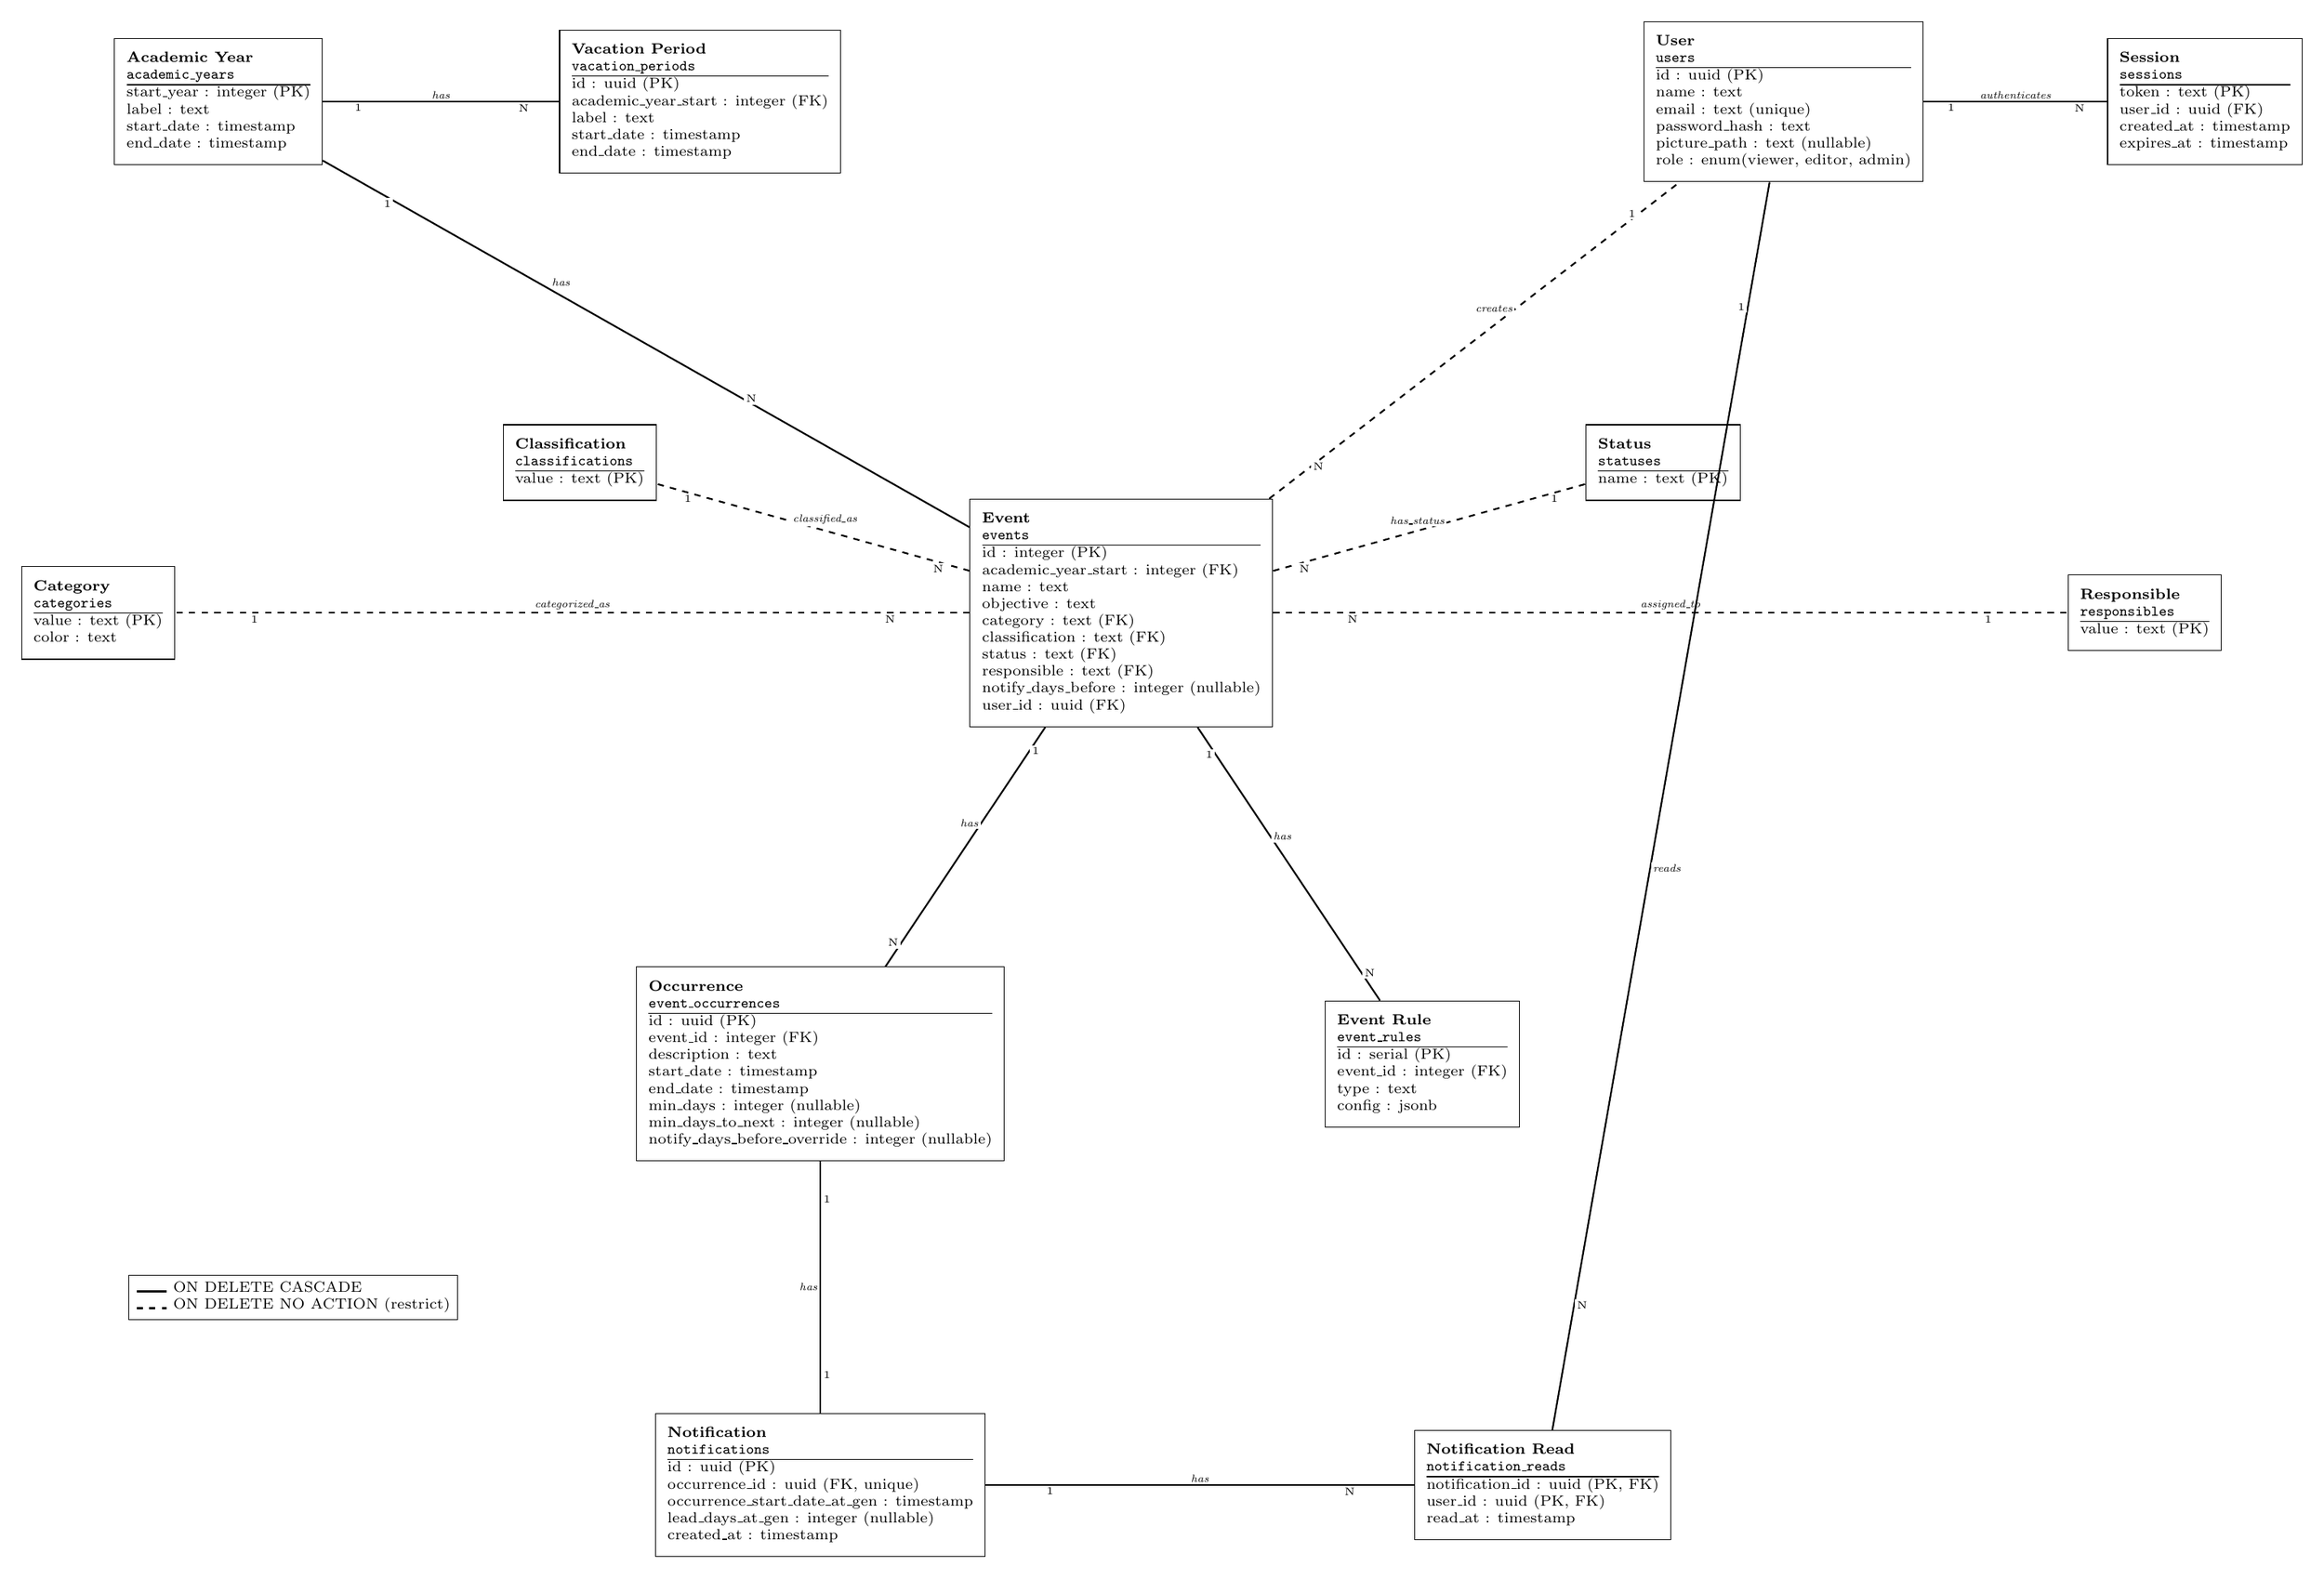
\begin{tikzpicture}[
    erentity/.style={draw, rectangle, align=left, font=\scriptsize, inner sep=2mm, fill=white},
    cascade/.style={thick},
    restrict/.style={thick, dashed},
    card/.style={fill=white, inner sep=1pt, font=\tiny},
    rel/.style={fill=white, inner sep=1pt, font=\tiny\itshape},
]

% --- entities, with full attribute lists ---
% Note: no three entities share both the same x and the same y-alignment as
% any drawn edge, so that no relationship line passes through an unrelated
% entity box (classifications/statuses are offset in y from the
% categories-event-responsibles spine for this reason).
\node[erentity] (academicyears) at (-15,9) {%
  \begin{tabular}{@{}l@{}}
    \textbf{Academic Year} \\ {\scriptsize\ttfamily academic\_years} \\ \hline
    start\_year : integer (PK) \\
    label : text \\
    start\_date : timestamp \\
    end\_date : timestamp
  \end{tabular}%
};

\node[erentity] (vacationperiods) at (-7,9) {%
  \begin{tabular}{@{}l@{}}
    \textbf{Vacation Period} \\ {\scriptsize\ttfamily vacation\_periods} \\ \hline
    id : uuid (PK) \\
    academic\_year\_start : integer (FK) \\
    label : text \\
    start\_date : timestamp \\
    end\_date : timestamp
  \end{tabular}%
};

\node[erentity] (users) at (11,9) {%
  \begin{tabular}{@{}l@{}}
    \textbf{User} \\ {\scriptsize\ttfamily users} \\ \hline
    id : uuid (PK) \\
    name : text \\
    email : text (unique) \\
    password\_hash : text \\
    picture\_path : text (nullable) \\
    role : enum(viewer, editor, admin)
  \end{tabular}%
};

\node[erentity] (sessions) at (18,9) {%
  \begin{tabular}{@{}l@{}}
    \textbf{Session} \\ {\scriptsize\ttfamily sessions} \\ \hline
    token : text (PK) \\
    user\_id : uuid (FK) \\
    created\_at : timestamp \\
    expires\_at : timestamp
  \end{tabular}%
};

\node[erentity] (categories) at (-17,0.5) {%
  \begin{tabular}{@{}l@{}}
    \textbf{Category} \\ {\scriptsize\ttfamily categories} \\ \hline
    value : text (PK) \\
    color : text
  \end{tabular}%
};

\node[erentity] (classifications) at (-9,3) {%
  \begin{tabular}{@{}l@{}}
    \textbf{Classification} \\ {\scriptsize\ttfamily classifications} \\ \hline
    value : text (PK)
  \end{tabular}%
};

\node[erentity] (event) at (0,0.5) {%
  \begin{tabular}{@{}l@{}}
    \textbf{Event} \\ {\scriptsize\ttfamily events} \\ \hline
    id : integer (PK) \\
    academic\_year\_start : integer (FK) \\
    name : text \\
    objective : text \\
    category : text (FK) \\
    classification : text (FK) \\
    status : text (FK) \\
    responsible : text (FK) \\
    notify\_days\_before : integer (nullable) \\
    user\_id : uuid (FK)
  \end{tabular}%
};

\node[erentity] (statuses) at (9,3) {%
  \begin{tabular}{@{}l@{}}
    \textbf{Status} \\ {\scriptsize\ttfamily statuses} \\ \hline
    name : text (PK)
  \end{tabular}%
};

\node[erentity] (responsibles) at (17,0.5) {%
  \begin{tabular}{@{}l@{}}
    \textbf{Responsible} \\ {\scriptsize\ttfamily responsibles} \\ \hline
    value : text (PK)
  \end{tabular}%
};

\node[erentity] (occurrences) at (-5,-7) {%
  \begin{tabular}{@{}l@{}}
    \textbf{Occurrence} \\ {\scriptsize\ttfamily event\_occurrences} \\ \hline
    id : uuid (PK) \\
    event\_id : integer (FK) \\
    description : text \\
    start\_date : timestamp \\
    end\_date : timestamp \\
    min\_days : integer (nullable) \\
    min\_days\_to\_next : integer (nullable) \\
    notify\_days\_before\_override : integer (nullable)
  \end{tabular}%
};

\node[erentity] (rules) at (5,-7) {%
  \begin{tabular}{@{}l@{}}
    \textbf{Event Rule} \\ {\scriptsize\ttfamily event\_rules} \\ \hline
    id : serial (PK) \\
    event\_id : integer (FK) \\
    type : text \\
    config : jsonb
  \end{tabular}%
};

\node[erentity] (notifications) at (-5,-14) {%
  \begin{tabular}{@{}l@{}}
    \textbf{Notification} \\ {\scriptsize\ttfamily notifications} \\ \hline
    id : uuid (PK) \\
    occurrence\_id : uuid (FK, unique) \\
    occurrence\_start\_date\_at\_gen : timestamp \\
    lead\_days\_at\_gen : integer (nullable) \\
    created\_at : timestamp
  \end{tabular}%
};

\node[erentity] (notificationreads) at (7,-14) {%
  \begin{tabular}{@{}l@{}}
    \textbf{Notification Read} \\ {\scriptsize\ttfamily notification\_reads} \\ \hline
    notification\_id : uuid (PK, FK) \\
    user\_id : uuid (PK, FK) \\
    read\_at : timestamp
  \end{tabular}%
};

% --- relationships ---
\draw[cascade] (academicyears) -- (vacationperiods) node[rel, midway, above] {has} node[card, pos=0.15, below] {1} node[card, pos=0.85, below] {N};
\draw[cascade] (academicyears) -- (event) node[rel, pos=0.35, above right] {has} node[card, pos=0.1, below] {1} node[card, pos=0.65, right] {N};

\draw[restrict] (event) -- (categories) node[rel, midway, above] {categorized\_as} node[card, pos=0.1, below] {N} node[card, pos=0.9, below] {1};
\draw[restrict] (event) -- (classifications) node[rel, midway, above, xshift=2mm] {classified\_as} node[card, pos=0.1, below] {N} node[card, pos=0.9, below] {1};
\draw[restrict] (event) -- (statuses) node[rel, midway, above, xshift=-2mm] {has\_status} node[card, pos=0.1, below] {N} node[card, pos=0.9, below] {1};
\draw[restrict] (event) -- (responsibles) node[rel, midway, above] {assigned\_to} node[card, pos=0.1, below] {N} node[card, pos=0.9, below] {1};

\draw[restrict] (event) -- (users) node[rel, pos=0.6, left] {creates} node[card, pos=0.1, right] {N} node[card, pos=0.9, left] {1};
\draw[cascade] (users) -- (sessions) node[rel, midway, above] {authenticates} node[card, pos=0.15, below] {1} node[card, pos=0.85, below] {N};

\draw[cascade] (event) -- (occurrences) node[rel, pos=0.4, left] {has} node[card, pos=0.1, right] {1} node[card, pos=0.9, left] {N};
\draw[cascade] (event) -- (rules) node[rel, pos=0.4, right] {has} node[card, pos=0.1, left] {1} node[card, pos=0.9, right] {N};

\draw[cascade] (occurrences) -- (notifications) node[rel, midway, left] {has} node[card, pos=0.15, right] {1} node[card, pos=0.85, right] {1};
\draw[cascade] (notifications) -- (notificationreads) node[rel, midway, above] {has} node[card, pos=0.15, below] {1} node[card, pos=0.85, below] {N};
\draw[cascade] (users) -- (notificationreads) node[rel, pos=0.55, right] {reads} node[card, pos=0.1, left] {1} node[card, pos=0.9, right] {N};

% --- legend ---
\node[draw, align=left, font=\scriptsize, anchor=north west, fill=white] at (-16.5,-10.5) {
    \tikz{\draw[cascade] (0,0) -- (0.5,0);} ON DELETE CASCADE \\
    \tikz{\draw[restrict] (0,0) -- (0.5,0);} ON DELETE NO ACTION (restrict)
};
\end{tikzpicture}%
}
\end{center}
\caption{Full Entity-Relationship Diagram with column-level attributes, derived from the Drizzle schema.}\label{fig:er-diagram-full}
\end{figure}
\end{landscape}
